\let\negmedspace\undefined
\let\negthickspace\undefined
\documentclass[journal]{IEEEtran}
\usepackage[a5paper, margin=10mm, onecolumn]{geometry}
%\usepackage{lmodern} % Ensure lmodern is loaded for pdflatex
\usepackage{tfrupee} % Include tfrupee package

\setlength{\headheight}{1cm} % Set the height of the header box
\setlength{\headsep}{0mm}     % Set the distance between the header box and the top of the text

\usepackage{gvv-book}
\usepackage{gvv}
\usepackage{cite}
\usepackage{amsmath,amssymb,amsfonts,amsthm}
\usepackage{algorithmic}
\usepackage{graphicx}
\usepackage{textcomp}
\usepackage{xcolor}
\usepackage{txfonts}
\usepackage{listings}
\usepackage{enumitem}
\usepackage{mathtools}
\usepackage{gensymb}
\usepackage{comment}
\usepackage[breaklinks=true]{hyperref}
\usepackage{tkz-euclide} 
\usepackage{listings}
% \usepackage{gvv}                                        
\def\inputGnumericTable{}                                 
\usepackage[latin1]{inputenc}                                
\usepackage{color}                                            
\usepackage{array}                                            
\usepackage{longtable}                                       
\usepackage{calc}                                             
\usepackage{multirow}                                         
\usepackage{hhline}                                           
\usepackage{ifthen}                                           
\usepackage{lscape}
\begin{document}
\bibliographystyle{IEEEtran}
\title{2.3.5}
\author{EE25BTECH11002 - Achat Parth Kalpesh }
{\let\newpage\relax\maketitle}
\renewcommand{\thefigure}{\theenumi}
\renewcommand{\thetable}{\theenumi}
\setlength{\intextsep}{10pt} % Space between text and floats
\numberwithin{equation}{enumi}
\numberwithin{figure}{enumi}
\renewcommand{\thetable}{\theenumi}
\parindent 0px

\textbf{Question:}\\
Find the angle between the line $\vec{r} = \brak{\hat{i} - \hat{j} + \hat{k}} + \lambda\brak{3\hat{i} - \hat{j} + 2\hat{k}}$ and the plane $\vec{r} \cdot \brak{\hat{i} + \hat{j} + \hat{k}} = 3$.

\textbf{Solution:}\\
From the given equations, we can identify the direction vector of the line,
$\vec{d}$, and the normal vector of the plane, $\vec{n}$.

\begin{align} 
\label{eq:d_vec}
\vec{d} = \myvec{3\\-1\\2} \\
\label{eq:n_vec}
\vec{n} = \myvec{1\\1\\1}
\end{align}


If $\theta$ is the angle between the line and the plane, then the angle between the line's direction vector $\vec{d}$ and the plane's normal vector $\vec{n}$ is $90\degree - \theta$. The formula to calculate the angle $\theta$ is:
\begin{align}
\theta = \sin^{-1}\brak{\frac{\abs{\vec{n}^\top\vec{d}}}{\norm{\vec{d}} \norm{\vec{n}}}}
\end{align}

Substituting the vectors $\vec{d}$ and $\vec{n}$ into this formula:
\begin{align}
\theta &= \sin^{-1}\brak{\frac{\abs{\myvec{1&1&1}\myvec{3\\-1\\2}}}{\norm{\myvec{3\\-1\\2}}\norm{\myvec{1\\1\\1}}}} \\
&= \sin^{-1} \brak{\frac{\abs{\brak{3}\brak{1} + \brak{-1}\brak{1} + \brak{2}\brak{1}}}{\sqrt{3^2 + \brak{-1}^2 + 2^2}\sqrt{1^2 + 1^2 + 1^2}}} \\
&= \sin^{-1}\brak{\frac{\abs{3-1+2}}{\sqrt{9+1+4}\sqrt{3}}} \\
&= \sin^{-1}\brak{\frac{\abs{4}}{\sqrt{14}\sqrt{3}}} \\
&= \sin^{-1}\brak{\frac{4}{\sqrt{42}}}
\end{align}


So, the angle $\theta$ is:
\begin{align}
\theta = \sin^{-1}\brak{\frac{4}{\sqrt{42}}}
\end{align}


This is approximately $37.98\degree$

\begin{figure}[h]
    \centering
    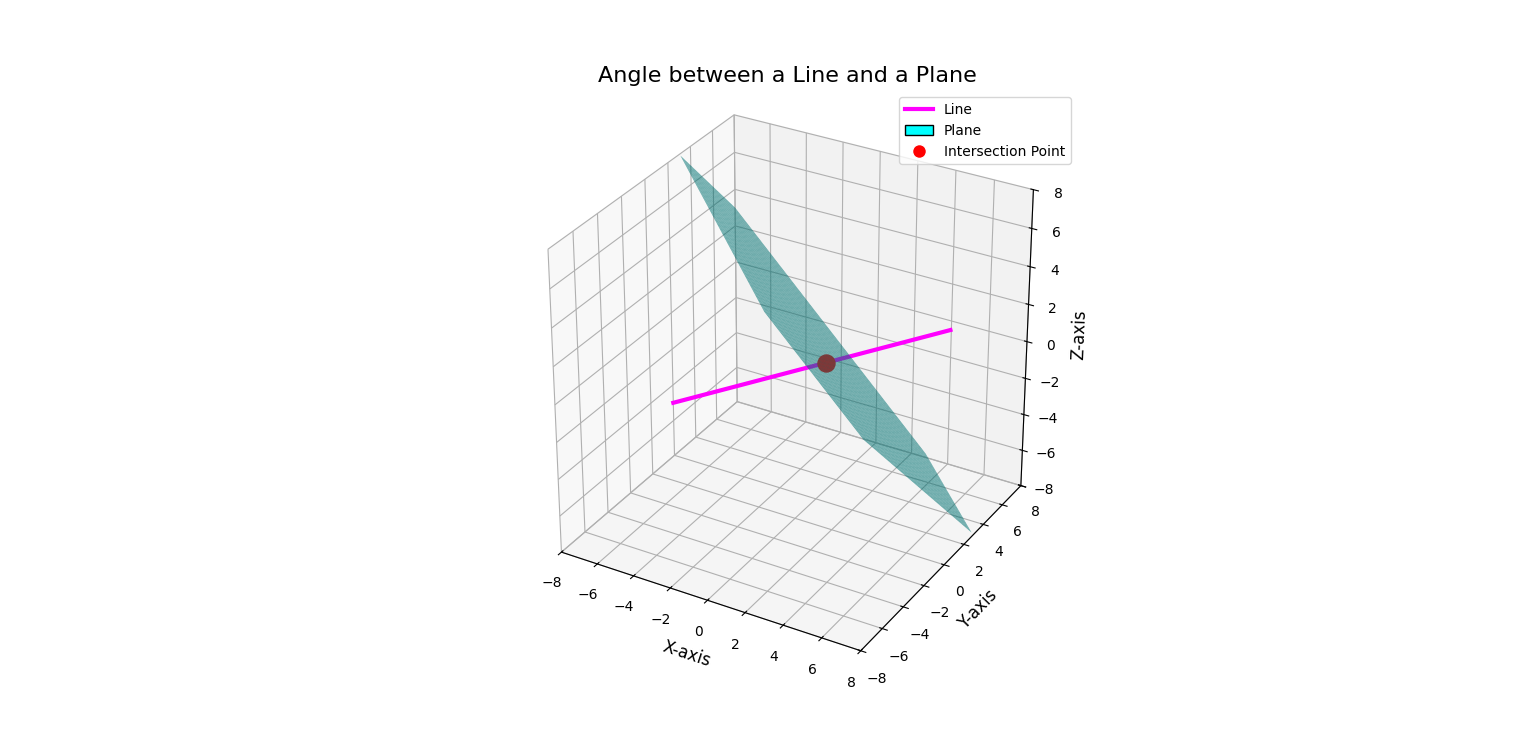
\includegraphics[width=\columnwidth]{figs/pure_python.png}
    \caption{Graph}
    \label{fig:fig}
 \end{figure}


\end{document}